
\PassOptionsToPackage{table}{xcolor}

\documentclass[sigconf%
,natbib=true%
]{acmart}

\usepackage{balance}

\copyrightyear{2021}
\acmYear{2021}
\setcopyright{acmlicensed}\acmConference[VINCI '21]{The 14th International Symposium on Visual Information Communication and Interaction}{September 6--8, 2021}{Potsdam, Germany}
\acmBooktitle{The 14th International Symposium on Visual Information Communication and Interaction (VINCI '21), September 6--8, 2021, Potsdam, Germany}
\acmPrice{15.00}
\acmDOI{10.1145/3481549.3481568}
\acmISBN{978-1-4503-8647-0/21/09}

\usepackage[utf8]{inputenc}
\usepackage{tabularx}
\usepackage{csquotes}
\usepackage{tikz}
\usetikzlibrary{positioning}
\usepackage{amsmath}
\usepackage{calc}
\usepackage{eurosym}

\usepackage[ruled,vlined,linesnumbered]{algorithm2e}
\usepackage{algpseudocode}
\SetAlFnt{\small}
\SetAlCapFnt{\footnotesize}
\SetAlCapNameFnt{\footnotesize}

\usepackage{eso-pic}
\AddToShipoutPictureFG{\AtPageLowerLeft{\put(\LenToUnit{0.5\paperwidth},\LenToUnit{6mm}){\makebox[0pt][c]{\fontsize{6.5}{8}\selectfont\color{gray}Author's revised version (2026-11-10). Version of record: https://doi.org/10.1145/3481549.3481568}}}}

\begin{document}

\title[Interactive Simulation and Visualization of Long-Term, ETF-based Investment Strategies]{Interactive Simulation and Visualization of\texorpdfstring{\\}{ }Long-Term, ETF-based Investment Strategies}

\author{Martin B{\"u}{\ss}emeyer}
\affiliation{%
	\institution{Hasso Plattner Institute, Digital Engineering Faculty}
	\country{University of Potsdam, Germany}
}
\author{Daniel Limberger}
\orcid{0000-0002-9111-4809}
\affiliation{%
\institution{Hasso Plattner Institute, Digital Engineering Faculty}
\country{University of Potsdam, Germany}
}
\author{Willy Scheibel}
\orcid{0000-0002-7885-9857}
\affiliation{%
  \institution{Hasso Plattner Institute, Digital Engineering Faculty}
  \country{University of Potsdam, Germany}
}
\author{J{\"u}rgen D{\"o}llner}
\affiliation{%
  \institution{Hasso Plattner Institute, Digital Engineering Faculty}
  \country{University of Potsdam, Germany}
}

\renewcommand{\shortauthors}{M.~B{\"u}{\ss}emeyer, D.~Limberger, W.~Scheibel, J.~D{\"o}llner}

\begin{abstract}
    Personal, long-term investment products, especially ones for retirement savings, require thorough understanding to use them profitably.
    Even simple savings plans based on exchange-traded funds (ETFs) are subject to many variables and uncertainties to be considered for expected and planned-upon returns.
    We present an interactive simulation of an ETF-based savings plan that combines forecasts, risk awareness, taxes and costs, inflation, and dynamic inflows and outflows into a single visualization.
    The visualization consists of four parts: 
        a form-fill interface for configuration, 
        a savings and payout simulation, 
        a cash flow chart, 
        and a savings chart.
    Based on a specific use case, we discuss how private investors can benefit from using our visualization after a short training period.
\end{abstract}

\begin{CCSXML}
	<ccs2012>
	<concept>
	<concept_id>10003120.10003145.10003147.10010923</concept_id>
	<concept_desc>Human-centered computing~Information visualization</concept_desc>
	<concept_significance>300</concept_significance>
	</concept>
	</ccs2012>
\end{CCSXML}

\ccsdesc[300]{Human-centered computing~Information visualization}

\keywords{%
    \texorpdfstring{\spaceskip=0.8\fontdimen2\font plus 0.5\fontdimen3\font minus \fontdimen4\font}{}interactive visualization, 
    financial visualization, 
    401(k) plan visualization, 
    ETF savings plan visualization,
    retirement savings calculator}

\maketitle

\section{Introduction}
Pension entitlement is currently falling continuously due to the demographic change~\cite{wendel2016-retirement,borsch2012riester}. 
To make up for a gap in personal retirement provision, one can resort to offers from financial institutions. 
For example, \emph{Riester} in Germany~\cite{borsch2012riester, ubber28exchange} or the more widely known \emph{401(k)} plans in the USA~\cite{wolff2011transformation}.
The underlying strategies are often actively managed and produce unnecessary costs, while passive strategies tend to win over active strategies in the long run~\cite{kommer2018souveran}.
This is one of the reasons why passive investment strategies based on long-term saving plans using exchange-traded funds (ETFs) have become quite popular and gain more attraction in other countries.
Since most direct banks and brokers provide opportunities for regular, small investments in ETFs with reduced costs, it is fairly easy to minimize costs and administrative expenses in order to maximize savings.
\begin{figure}[t]
	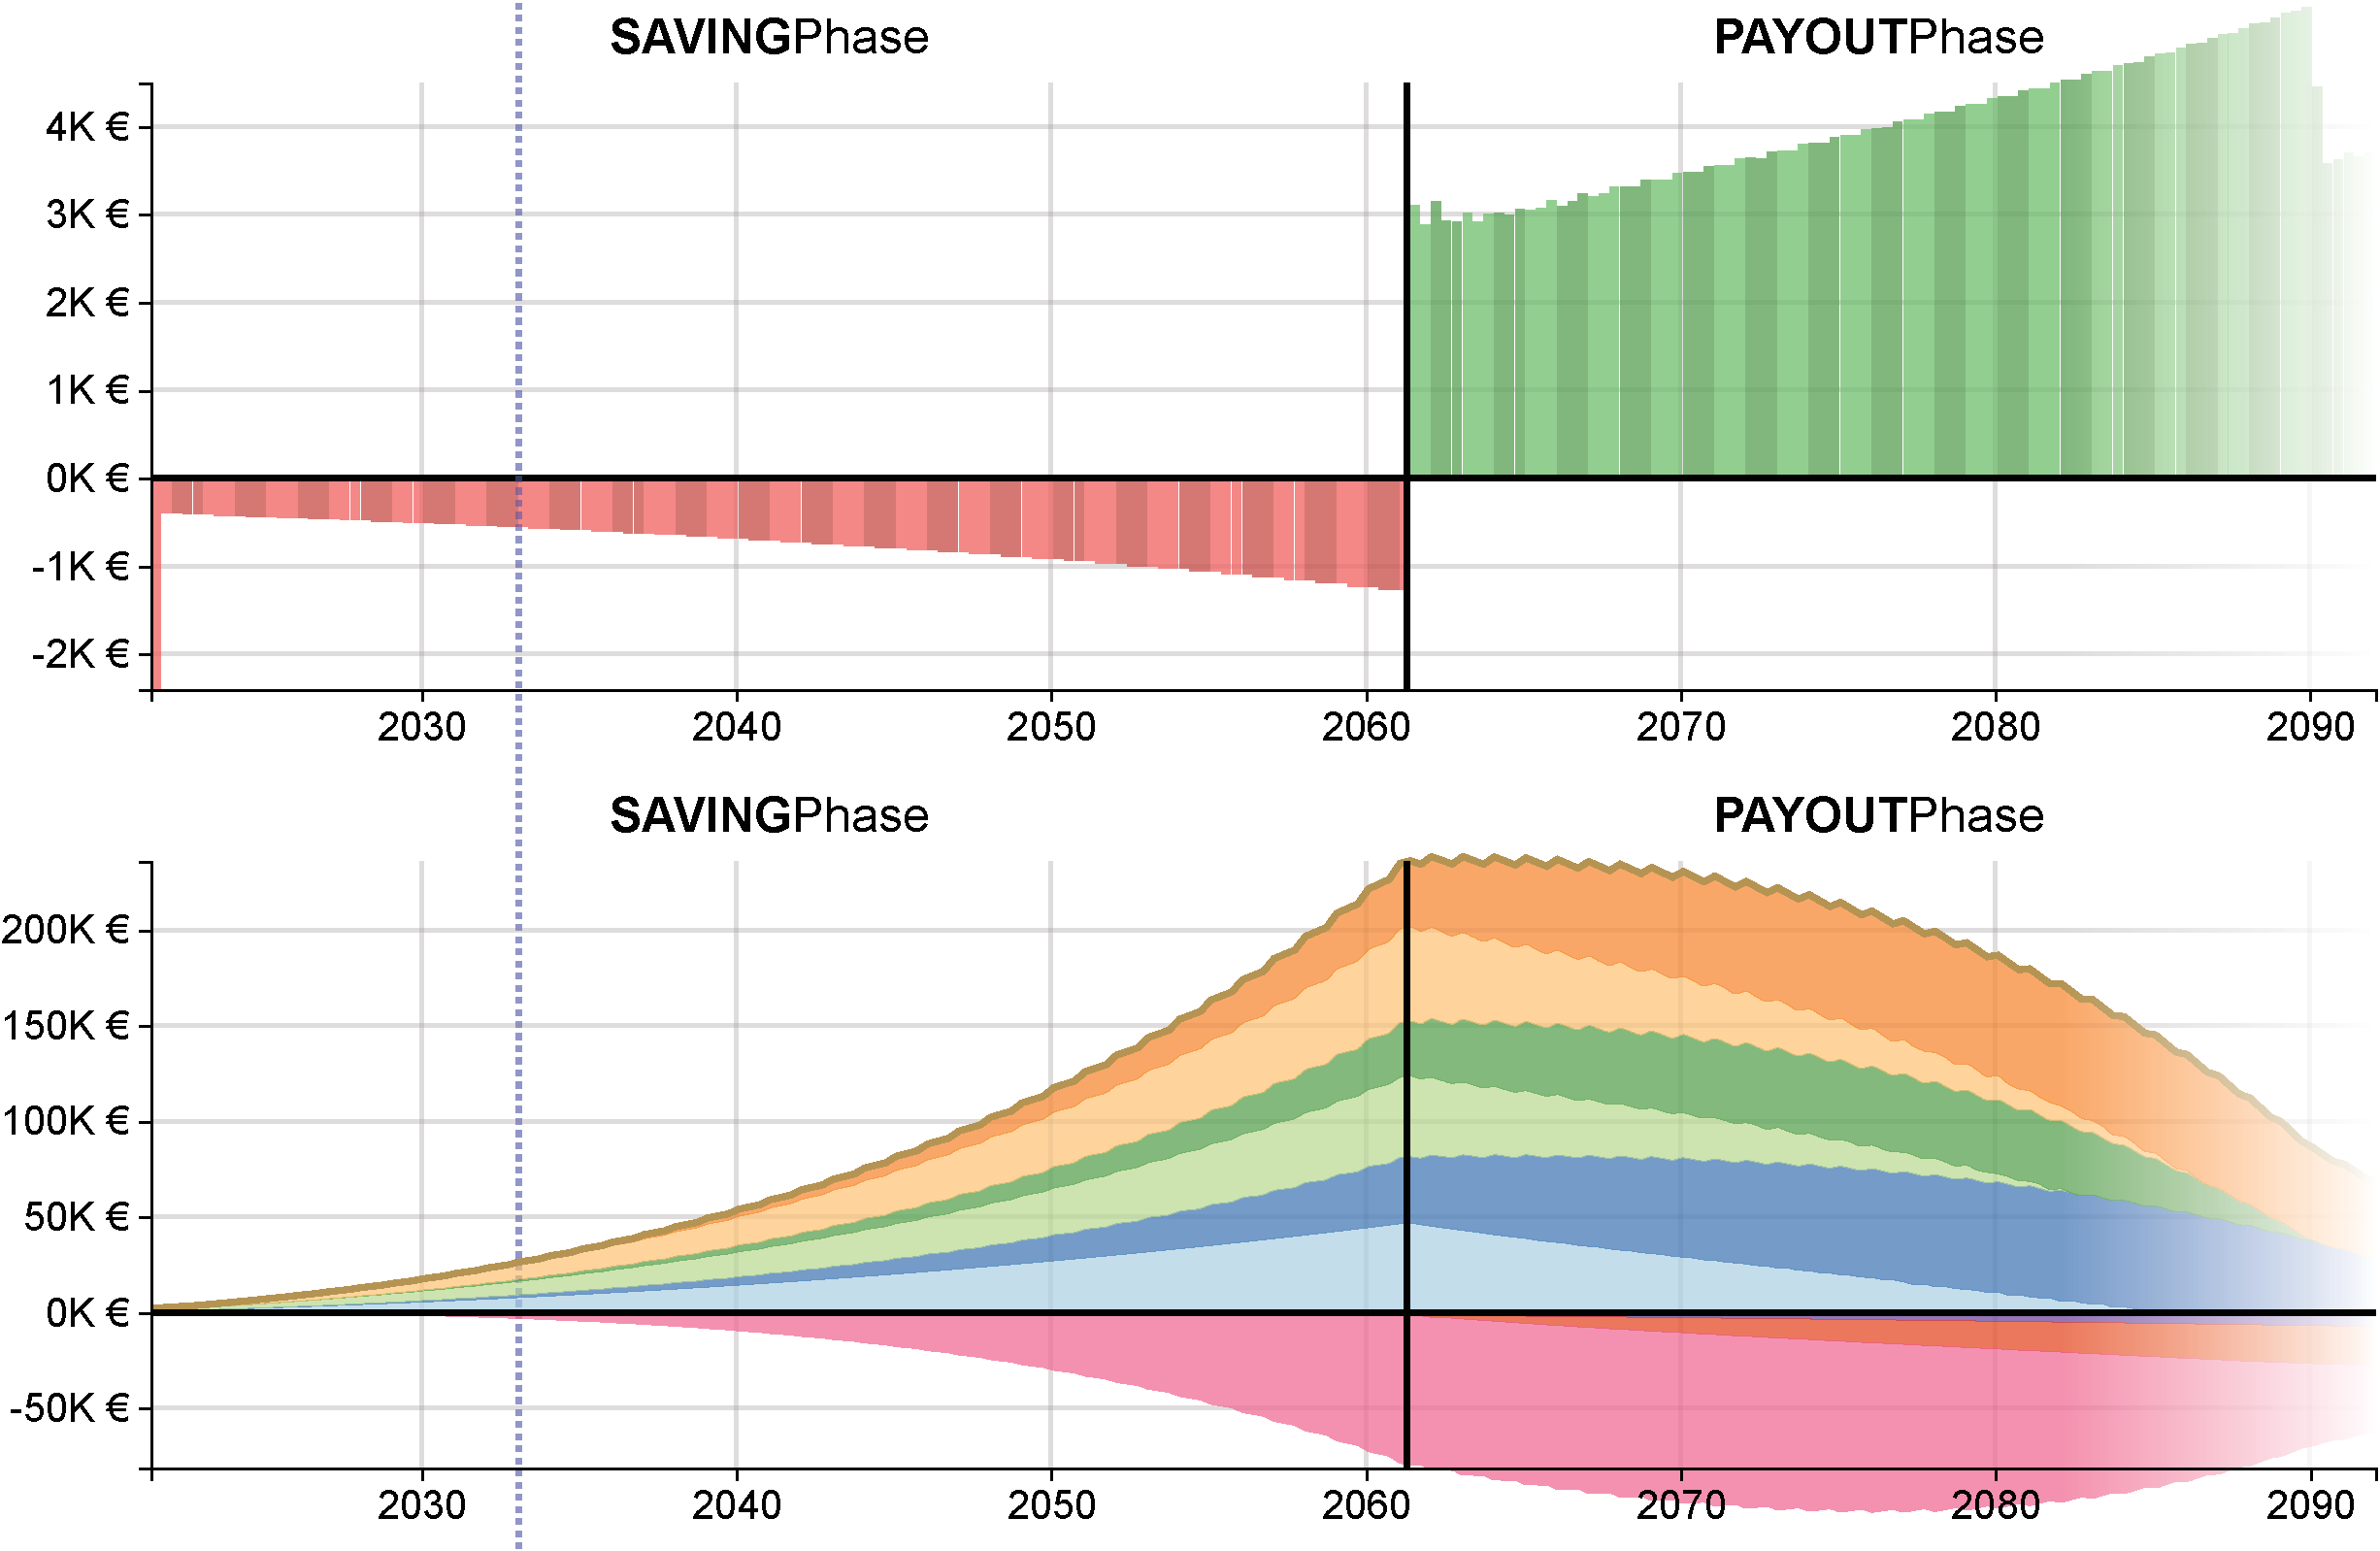
\includegraphics[width=\linewidth]{figures/teaser-v1.pdf}
    \caption{Our visualization of a plan with a dynamic \euro~100 monthly investment split into three accumulating ETFs. The cash flow chart (top) depicts the monthly investments and payouts. The depot chart (bottom) shows the simulated forecast of the savings, taxes (red), costs, and inflation (magenta) over a time-span of 40 (saving) plus 30 (payout) years.
    This shows, i.a., a dynamic payout of \euro~ 800 with the start of the pension is reasonably sustainable for at least 20 years.}
    \label{fig:teaser}
\end{figure}
The ETF investment system itself, however, is rather complicated and requires stock market literacy~\cite{balloch2014-literacy}.
Therein lies a fundamental conflict of interest, as forecasts from brokers or banks themselves are not designed to be transparent to the customer. 
In order to maximize incentives to create a depot, everything is kept as simple as possible.
This leads to over-simplified communication of costs, taxes, and idealized forecasts~\cite{devilliers2019-reframing}.
The main contributions of this work are
\begin{itemize}
    \item a savings plan simulation that takes growth, dividends, taxation, and transaction costs into account, and
    \item a visualization using a cash flow chart and a savings chart accounting for inflation, taxes, costs, etc.
\end{itemize}

\enquote{The most straightforward (and generic) approach to enhancing the value of an unknown outcome is to communicate concrete consequences}~\cite{wiener2008-framework}.
Thus, self-efficacy with regard to financial decision-making improves the likelihood that individuals follow the retirement strategy~\cite{lusardi2017-narratives}.
\enquote{[A] recent study found that less than 25\% of [American] individuals over the age of 50 succeeded at saving for retirement, often because they were unaware of fundamental economic concepts such as interest rate or inflation}~\cite{rudolph2009-finvis}.

We propose an interactive savings simulation and target non-experts to support decision-making on ETF-based saving plans~(\autoref{fig:teaser}).
We enable interactive examination of various aspects of a savings plan by making all calculations in real time and provide immediate visual feedback.
This allows users to (1) understand the interactions of parameters and risks during savings and payout phase, and to (2) identify scenarios that fit their own needs.
Our open-source prototype focuses on Germany's tax law (could be adapted to other countries) and is available at \href{https://etf-vis.net}{etf-vis.net}.

\section{Related Work}
\enquote{Financial literacy empowers people to craft their finances in a way that they are able to manage their everyday expenses, maintain an emergency fund, plan for children's education and prepare for their swift post-retirement years}~\cite{goyal2021-literacy}. 
This becomes more important since employers and the federal government forward the responsibility to the individual resident~\cite{lusardi2017-narratives}.
This literacy is understood in a broader sense and \enquote{[v]isualizations may be [...] [a] good approach for overcoming processing difficulties because they shift information processing to the perceptual system, improving understanding of the concept presented and allowing decision-makers to quickly learn from trends and patterns in the data}~\cite{lusardi2017-narratives}.
For example, visualization is used to get an overview of whole markets and publicly available finance data~\cite{wattenberg1999-stockmarket}, or underlying mechanics and consequences~\cite{fry2013-teaching}.
Visualization has also become available for a more personal use~\cite{huang2015-personal} and was used to assess and communicate risks for savings~\cite{rudolph2009-finvis}.
We were surprised to see how few tools for forecasting and visualizations are currently available for end users.
Those available, however, usually kept relevant factors like costs, inflation, and taxes out of consideration~\cite{saving_plan_extra_etf, saving_plan_black_rock}. 
Similar issues are present in user-driven visualizations that generalize across country borders and thus cost and taxation models~\cite{portfolio-charts} though they are more transparent in their simulations.  

There are several statistical models used for predicting stock markets. 
One prominent model is ARIMA.
However, research has shown that ARIMA only works in some cases for forecasting short-term periods~\cite{angadi2015-time, Cheng2020ApplicationOA, Mohamedashik2019StatisticalTF}. Moreover, we are aiming for long-term forecasting periods.
We can see that the market evolved in an exponential fashion during the last decades~\cite{leippold2016-index}. 
Thus, simpler regression models seem sufficient for our long-term forecasting.

\section{ETF Data \& Simulation}
Our simulation provides access to several ETFs, uses historical data for forecasting, and takes costs and German taxes into account.

\paragraph{Source Data}
We use historical data from Alphavantage to forecast prices.
Their API provides the average monthly closing value for the last five years of many well-known ETFs. 
Similar services are available from Yahoo Finance and Xignite.

\paragraph{German Costs and Taxation Model}
German citizens have a yearly exemption amount that can be used on investment gains to save taxes.
The tax amount is calculated by multiplying the gain by the partial exemption rate of $0.7$.
This prevents double taxation that would occur since the ETF owner has already paid taxes.
The tax rate is composed of capital gains tax and the solidarity contribution, which add up to $26.375\%$.
In Germany, the FIFO principle is prescribed for the sale of shares: the oldest shares are sold first. 
Since these are likely to have the highest profit, taxes due at the beginning of the payout period will be highest and decrease over time.
Accumulating and distributing ETFs differ in the way dividends are distributed and taxed.
Compared to distributing ETFs, accumulating ETFs reinvest the distribution automatically.
Instead of a dividend, the investor receives additional shares and no taxes are due. 
In 2018, the \emph{Vorabpauschale} (advance flat taxes) was introduced as part of an investment tax reform.
The taxes that need to be paid for a year's profit are limited by the expected profit. 
The expected profit is calculated by multiplying the amount invested by the \emph{base interest rate} and is discounted proportionately for each month of the year that has already passed.
Finally, the money distributed for the year is deducted from the resulting amount.
Thus, there are effectively no taxes for distributing ETFs.
Other costs arise from brokerage fees, usually a mix of fixed amounts and percentage costs.

\paragraph{Growth Model}
Statistical models like MA and ARIMA are used for short-term forecasts. 
Since we have to forecast far into the future, these models are not suitable.
Instead, models capturing general price development of recent decades seem to be sufficient.
Even though prices have continued to rise exponentially~\cite{leippold2016-index},
we decided to be pessimistic and assume a linear model inspired by~\cite{Nunno2014StockMP} in our simulation to avoid overly optimistic forecasts.
This can be easily replaced by an exponential model, if desired, or adjusted directly by means of a confidence score on the price development.

\begin{algorithm}[b]
    \SetAlCapSkip{-5cm}
    \SetAlgoSkip{}
	\footnotesize
	\selectfont
	\DontPrintSemicolon
	\SetKw{KwAnd}{and}
	\SetKwFunction{KwPush}{append}
	\SetKwFunction{KwBound}{binary\_search}
	$distributions \gets 0$\;
	$costs, investment \gets calculateCosts(investment)$\;
	$newShares \gets investment / currentPrice$\; 
	\If{$currentMonth == December$}{
	    \If{isDistributionModel}{
	        $distributions \gets distribution$\;
	        $taxes, distribution, taxFree \gets applyTaxes(distribution, taxFree)$\;
	    }
	    $newShares \gets newShares + distribution / currentPrice$\;
	    $expectedGain \gets calculateExpectedGain()$\;
        $vorabP \gets clamp(gain, 0, expectedGain - distributions)$\;
        $taxes \gets taxes + applyTaxes(max(0, vorabP - taxFree))$\;
	}
	$inflation \gets totalValue - totalValue * (1 - 0.02)^{yearsPassed}$\;
	\KwRet{newShares, costs, taxes, inflation}
	\selectfont
	\caption{Pseudo code of the calculation for a saving month.}%
	\label{alg:saving}
\end{algorithm}

\paragraph{Savings}
The savings phase starts with an optional starting capital and continues with a static or dynamic monthly amount. 
New shares are calculated by dividing the investment amount without costs by the current price. 
The \emph{Vorabpauschale} and payout of money take place in December. 
If a distributing strategy is used, taxes on returns are considered. 
The payout is then reinvested without additional costs and the \emph{Vorabpauschale} for this year is calculated.
Finally, the effectively lost amount of money caused by inflation is calculated.
This process is shown in Algorithm~\ref{alg:saving}.

\paragraph{Payouts}
During the payout phase, a specified monthly payout is withdrawn from the depot. 
For the distributing variant, payouts in December are not reinvested directly, but used for the monthly payout first.
Next, an iteration over the past investments is done according to the FIFO principle in order to withdraw the required amount. 
For each past investment, the gain is calculated and the occurring taxes (including the \emph{Vorabpauschale} in December) are deducted from the amount.
Finally, the occurring broker costs and the inflation are calculated.
The process is shown in Algorithm~\ref{alg:payout}.

\SetAlgoSkip{}
\begin{algorithm}[tb]
    \SetAlgoSkip{}
	\footnotesize
	\selectfont
	\DontPrintSemicolon
	\SetKw{KwAnd}{and}
	\SetKwFunction{KwPush}{append}
	\SetKwFunction{KwBound}{binary\_search}
	$receivedPayout \gets 0$\;
	\If{$currentMonth == December$}{
	    \If{isDistributionModel}{
	        $distributions \gets distribution$\;
	        $taxes, distribution \gets applyTaxes(distribution)$\;
	        $payout \gets payout - distribution$\;
	    }
	    \Else {
	        $newShares \gets distribution / currentPrice$\;
	    }
	}
	\For{oldestInvestment inv: until payout == 0}{
	    $gain \gets calculateGain(inv)$\;
	    $newTaxes, newPayout, taxFree \gets applyTaxes(gain, taxFree)$\;
	    $payout \gets payout - inv$\;
	    $receivedPayout \gets receivedPayout + (inv - newTaxes)$\;
	    $taxes \gets taxes + newTaxes$\;
	}
	\If{isDistributionModel}{
        $expectedGain \gets calculateExpectedGain()$\;
        $vorabP \gets clamp(gain, 0, expectedGain - distributions)$\;
        $taxes \gets taxes + applyTaxes(max(0, vorabP - taxFree))$\;
	}
	$costs, receivedPayout \gets calculateCosts(payout)$\;
	$inflation \gets totalValue - totalValue * (1 - 0.02)^{yearsPassed}$\;
	\KwRet{newShares, receivedPayout, costs, taxes, inflation}
	\selectfont
	\caption{Pseudo code of the calculation for a payout month.} %
	\label{alg:payout}
\end{algorithm}

\begin{figure}[b]
    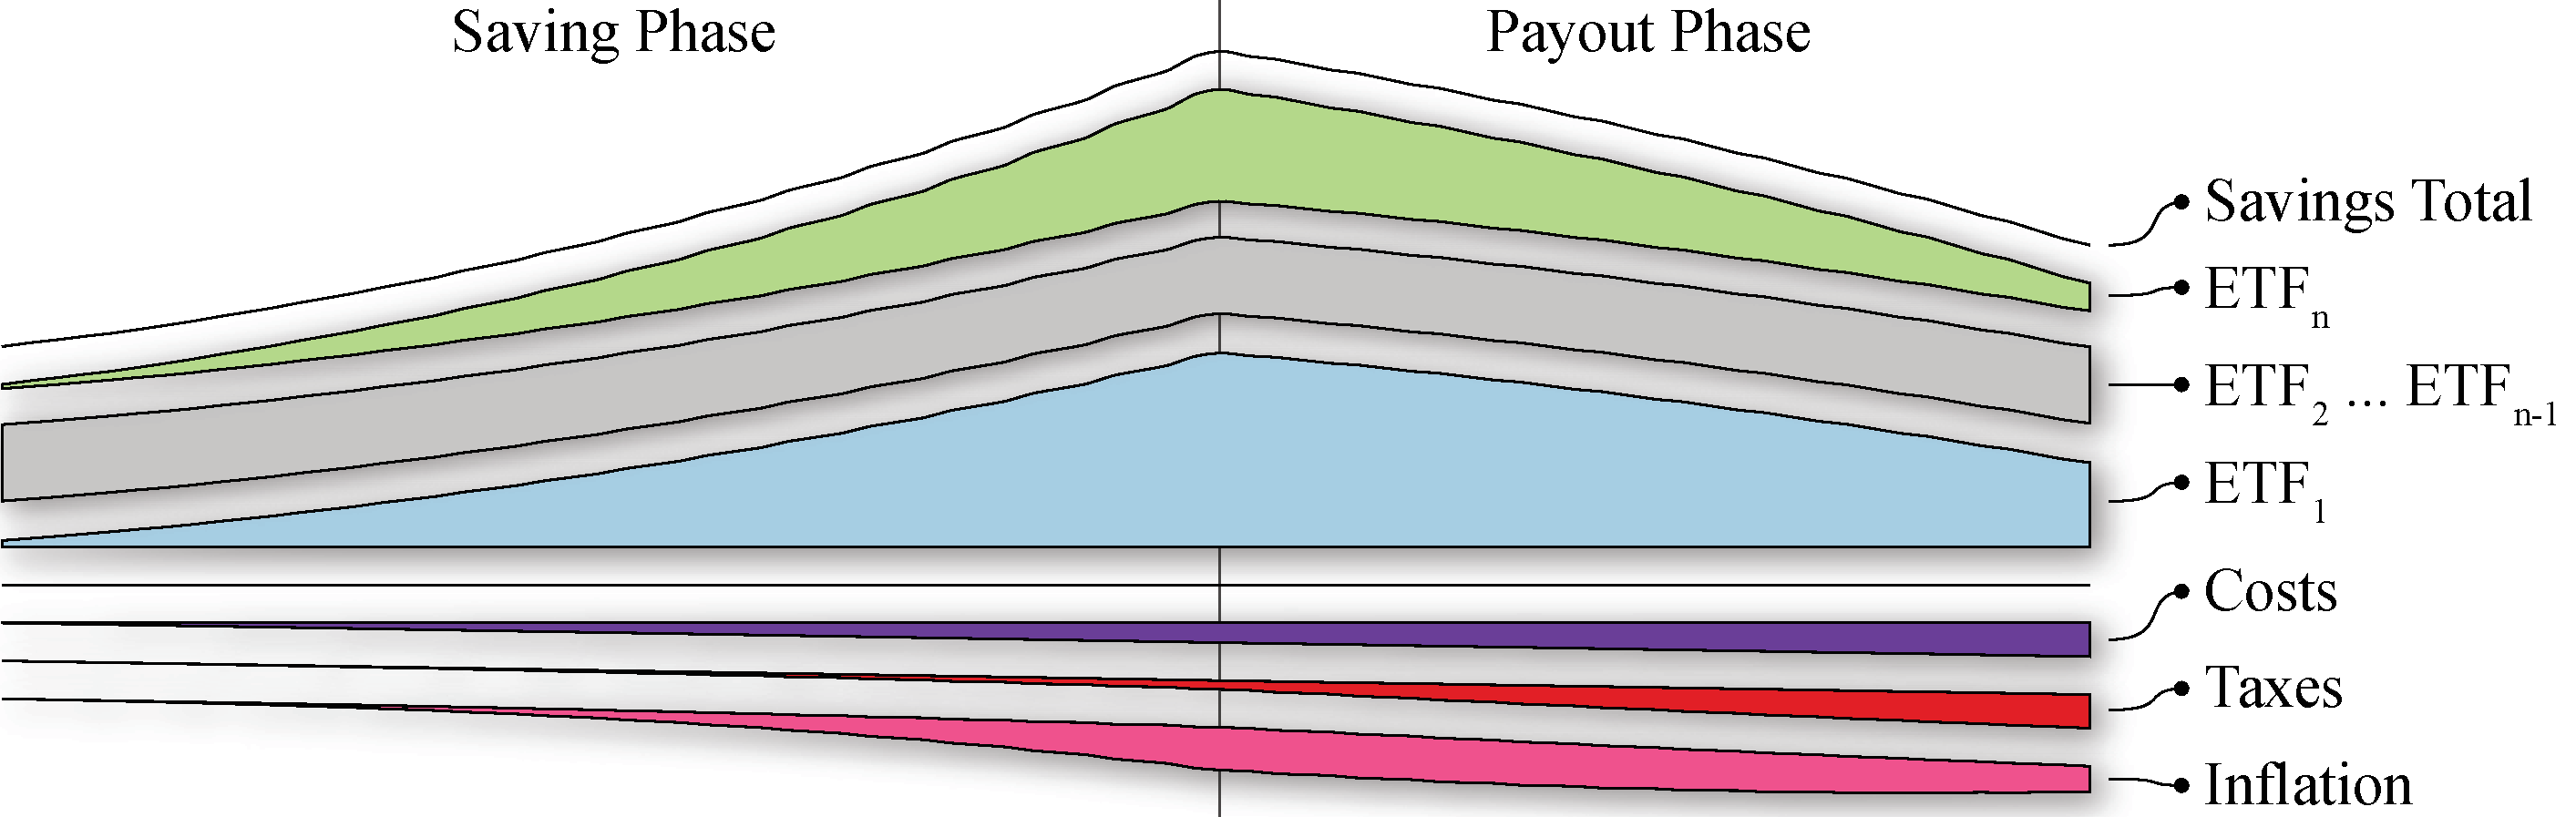
\includegraphics[width=\linewidth]{figures/composition.pdf}
    \caption{An explosion view depicting the composition of our depot view: 
    The upper part consists of $n$ ETFs with their values stacked on top of each other. 
    An additional line on top indicates the total saving. 
    The negative space consists of costs followed by taxes and inflation. 
    The x-axis splits positive and negative space and serves as semantic separator.}
    \label{fig:composition}
\end{figure}

\section{Visualization Technique}
The visualization features two charts, the cash flow and detail view, which are synced via a time-axis (x-axis).
The switch from saving to payout phase is indicated by a vertical line.
The end of the payout phase fades out to indicate inaccuracies in life expectancy.
The actual data at a certain time is printed on the right side when hovering over that point in time. 
The hovering is synced across both charts and is displayed via a vertical dashed line.
Next, the main user interface contains all parameterization options and is placed on the left.
The whole prototype is depicted in~\autoref{fig:visualization-full}.

\paragraph{Cash Flow Overview}
The cash flow chart visualizes the actual account movements using a bar chart.
The red bars indicate the investment, whereas the green bars represent the payout.
The payout already includes all fees and taxes. 
Each bar aggregates a certain configurable time period, e.g., a month or a quarterly period.

\paragraph{Detail View}
The detail view displays the depot value development and all associated negative effects: costs, taxes, and inflation.
A stacked area chart~(\autoref{fig:composition}) with a negative and positive part is used.
The positive part displays the value development of the ETFs.
Thereby, each ETF consists of two stacks. 
The lighter color shows the investment and the darker one is for the revenue. 
An additional line emphasizes the total value of the depot. 
The negative part consists of the accumulated costs (purple) and the accumulated taxes (red). 
Additionally, the inflation is added as a visual cue.
On the bottom of this chart, all actual values are listed in text form. 
They display the difference in the respective value to the previous parameter configuration with respect to the hovered point in time.
Moreover, a confidence area can be optionally added over the existing stacked areas. 
In this case, the borders of the confidence area are the total depot value that would incur when the minimum and maximum confidence would be used.
The middle line displays the currently selected confidence and is identical to the total value line when the confidence area is not displayed~(\autoref{fig:confidence}).

\begin{figure}[t]
    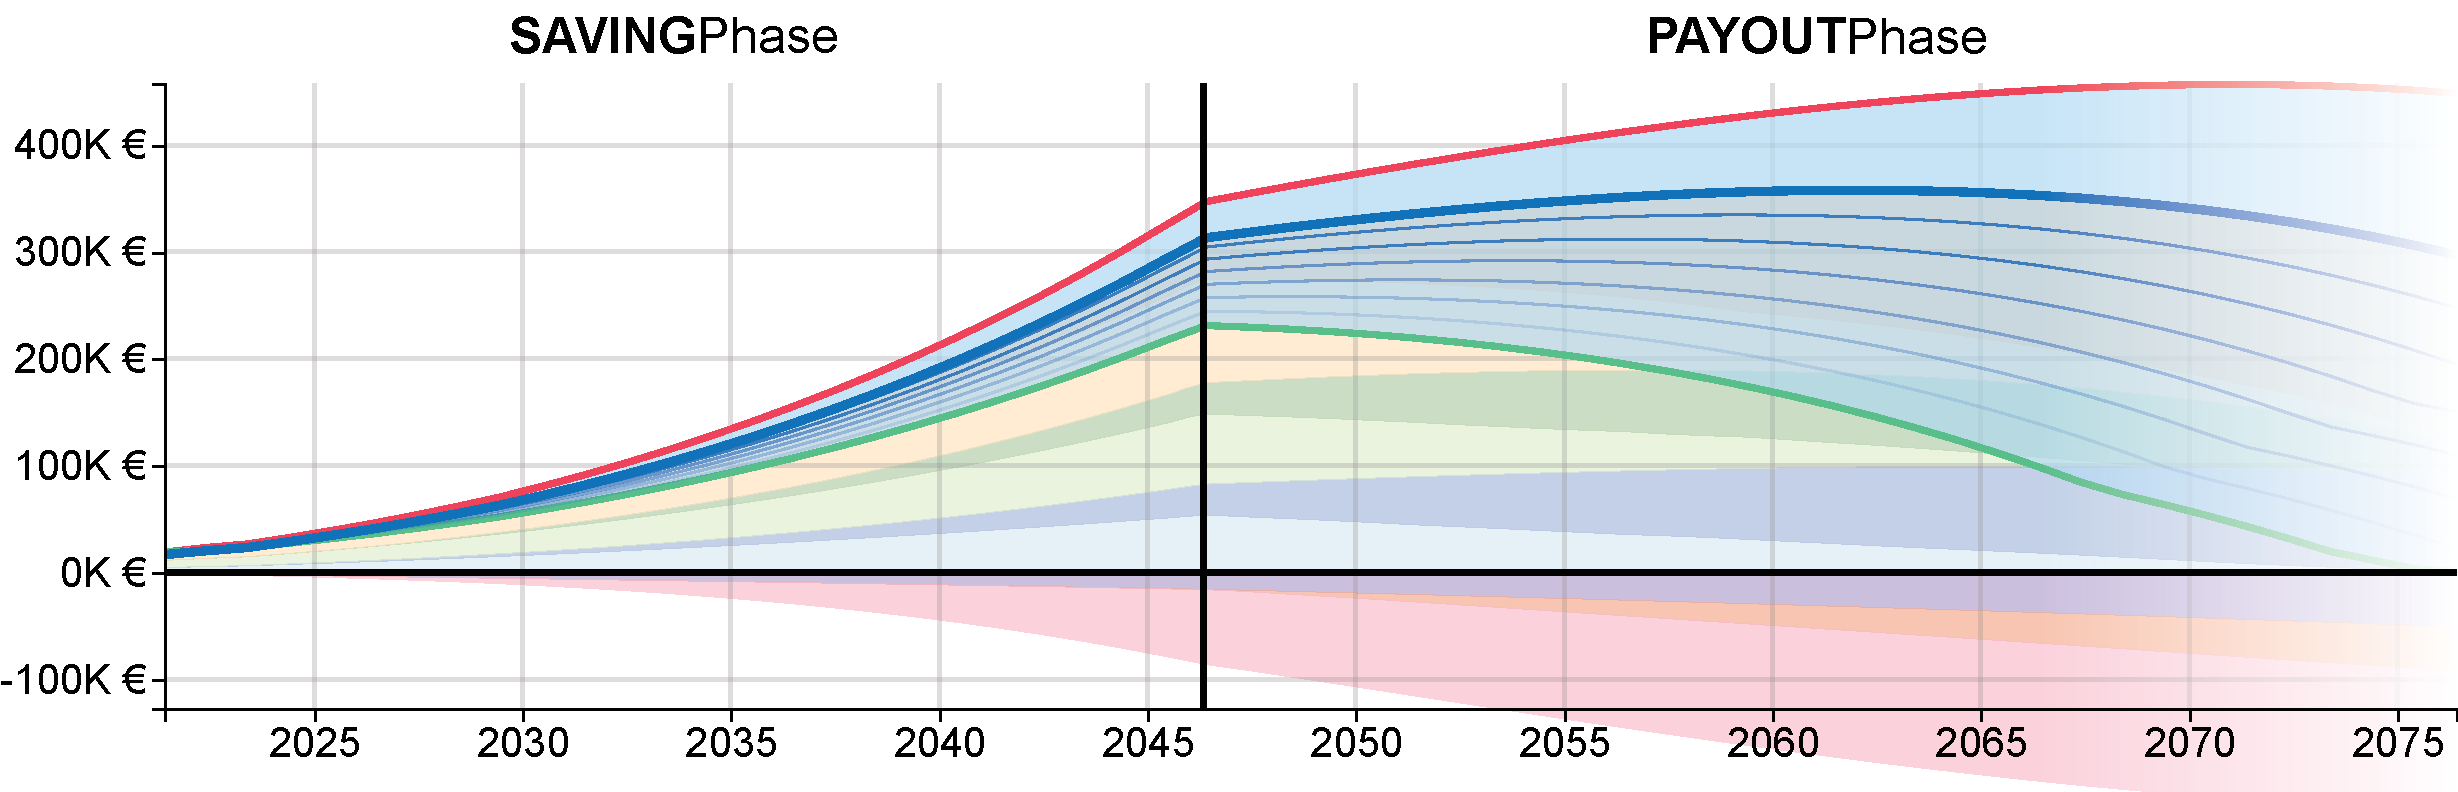
\includegraphics[width=\linewidth]{figures/confidence.pdf}
    \caption{The detail view when the confidence display option is activated. The standard stacked areas are more transparent and the confidence area is placed over it. The area displays the possible range of the total depot value. The area borders are enhanced by a green (maximal confidence) and red (minimal confidence) line. The used confidence interval is 0\%-100\%. The main blue line displays the confidence of the current configuration (30\%). Other lines are added artificially, displaying confidences in 10\% steps upwards.}
    \label{fig:confidence}
\end{figure}

\paragraph{Parameterization}
Parameters are divided into the categories money, time, cost, and visualization. 
In the money options the starting capital, monthly investment, and payout can be set. 
Investment and payout amounts can be set to dynamically increase on a yearly basis. 
The cost section gives control over the costs used for the saving and payout phase.
Furthermore, the time options specify the length of both phases by means of the current age, life expectancy, and years left until retirement.
The visualization options include ETF selection and confidence configuration used for forecasting.

\section{Use Case: Family Retirement Savings}
In this section, we (1) discuss the results of our prototypical simulation and visualization and (2) evaluate it by applying it to a certain use case and show the usefulness of the visualization.

\paragraph{Use Case: Family Retirement Savings}
Let's imagine a young family with one child. 
We assume a starting capital of \euro~ 1000, a monthly investment of \euro~ 100 and payout of \euro~ 1000. 
In order to compensate for inflation, both the investment and payout increase by $1\%$ per year. 
Additionally, the tax-free amount for a married couple is currently \euro~ 1602 and the accumulating version of the ETFs shall be used.
Moreover, the couple is around $25$ years old, will retire in $43$ years and has a life expectancy of $80$ years.
Their investment is equally spread across two standard ETFs: the S\,\&\,P~500 and MSCI~EM.
Furthermore, the family is assumed to already have an account at the bank ING which has relatively high investment costs with \euro~ 4.99 fixed costs and $0.25\%$ percentage costs.
The confidence is set to $100\%$ to minimize expectation.
The simulation predicts a depot value of \euro~ 161000 with overall costs of \euro~ 5200, \euro~ 0 taxes, and \euro~ 60000 effectively lost to inflation at the end of the saving phase.
Their depot lasts until 2084 which is one year before the expected lifetime. 
Until that date, \euro~ 8000 costs and \euro~ 7000 taxes will be paid. 
To ensure that the savings last until the expected lifetime, a cheaper broker with only $1\%$ percentage costs can be chosen to minimize the costs. 
This will result in \euro~ 3150 costs, \euro~ 8120 taxes and a leftover depot amount of \euro~ 15700 at the expected lifetime (still not enough though).
In this case, the visualization enables long-term planning and shows the impact of individual factors.
At best, it could lead to better future planning and decision-making. 
For example, changing the bank and increasing the monthly investment dynamically to minimize costs and allow for a buffer respectively. 

\begin{figure}[t]
    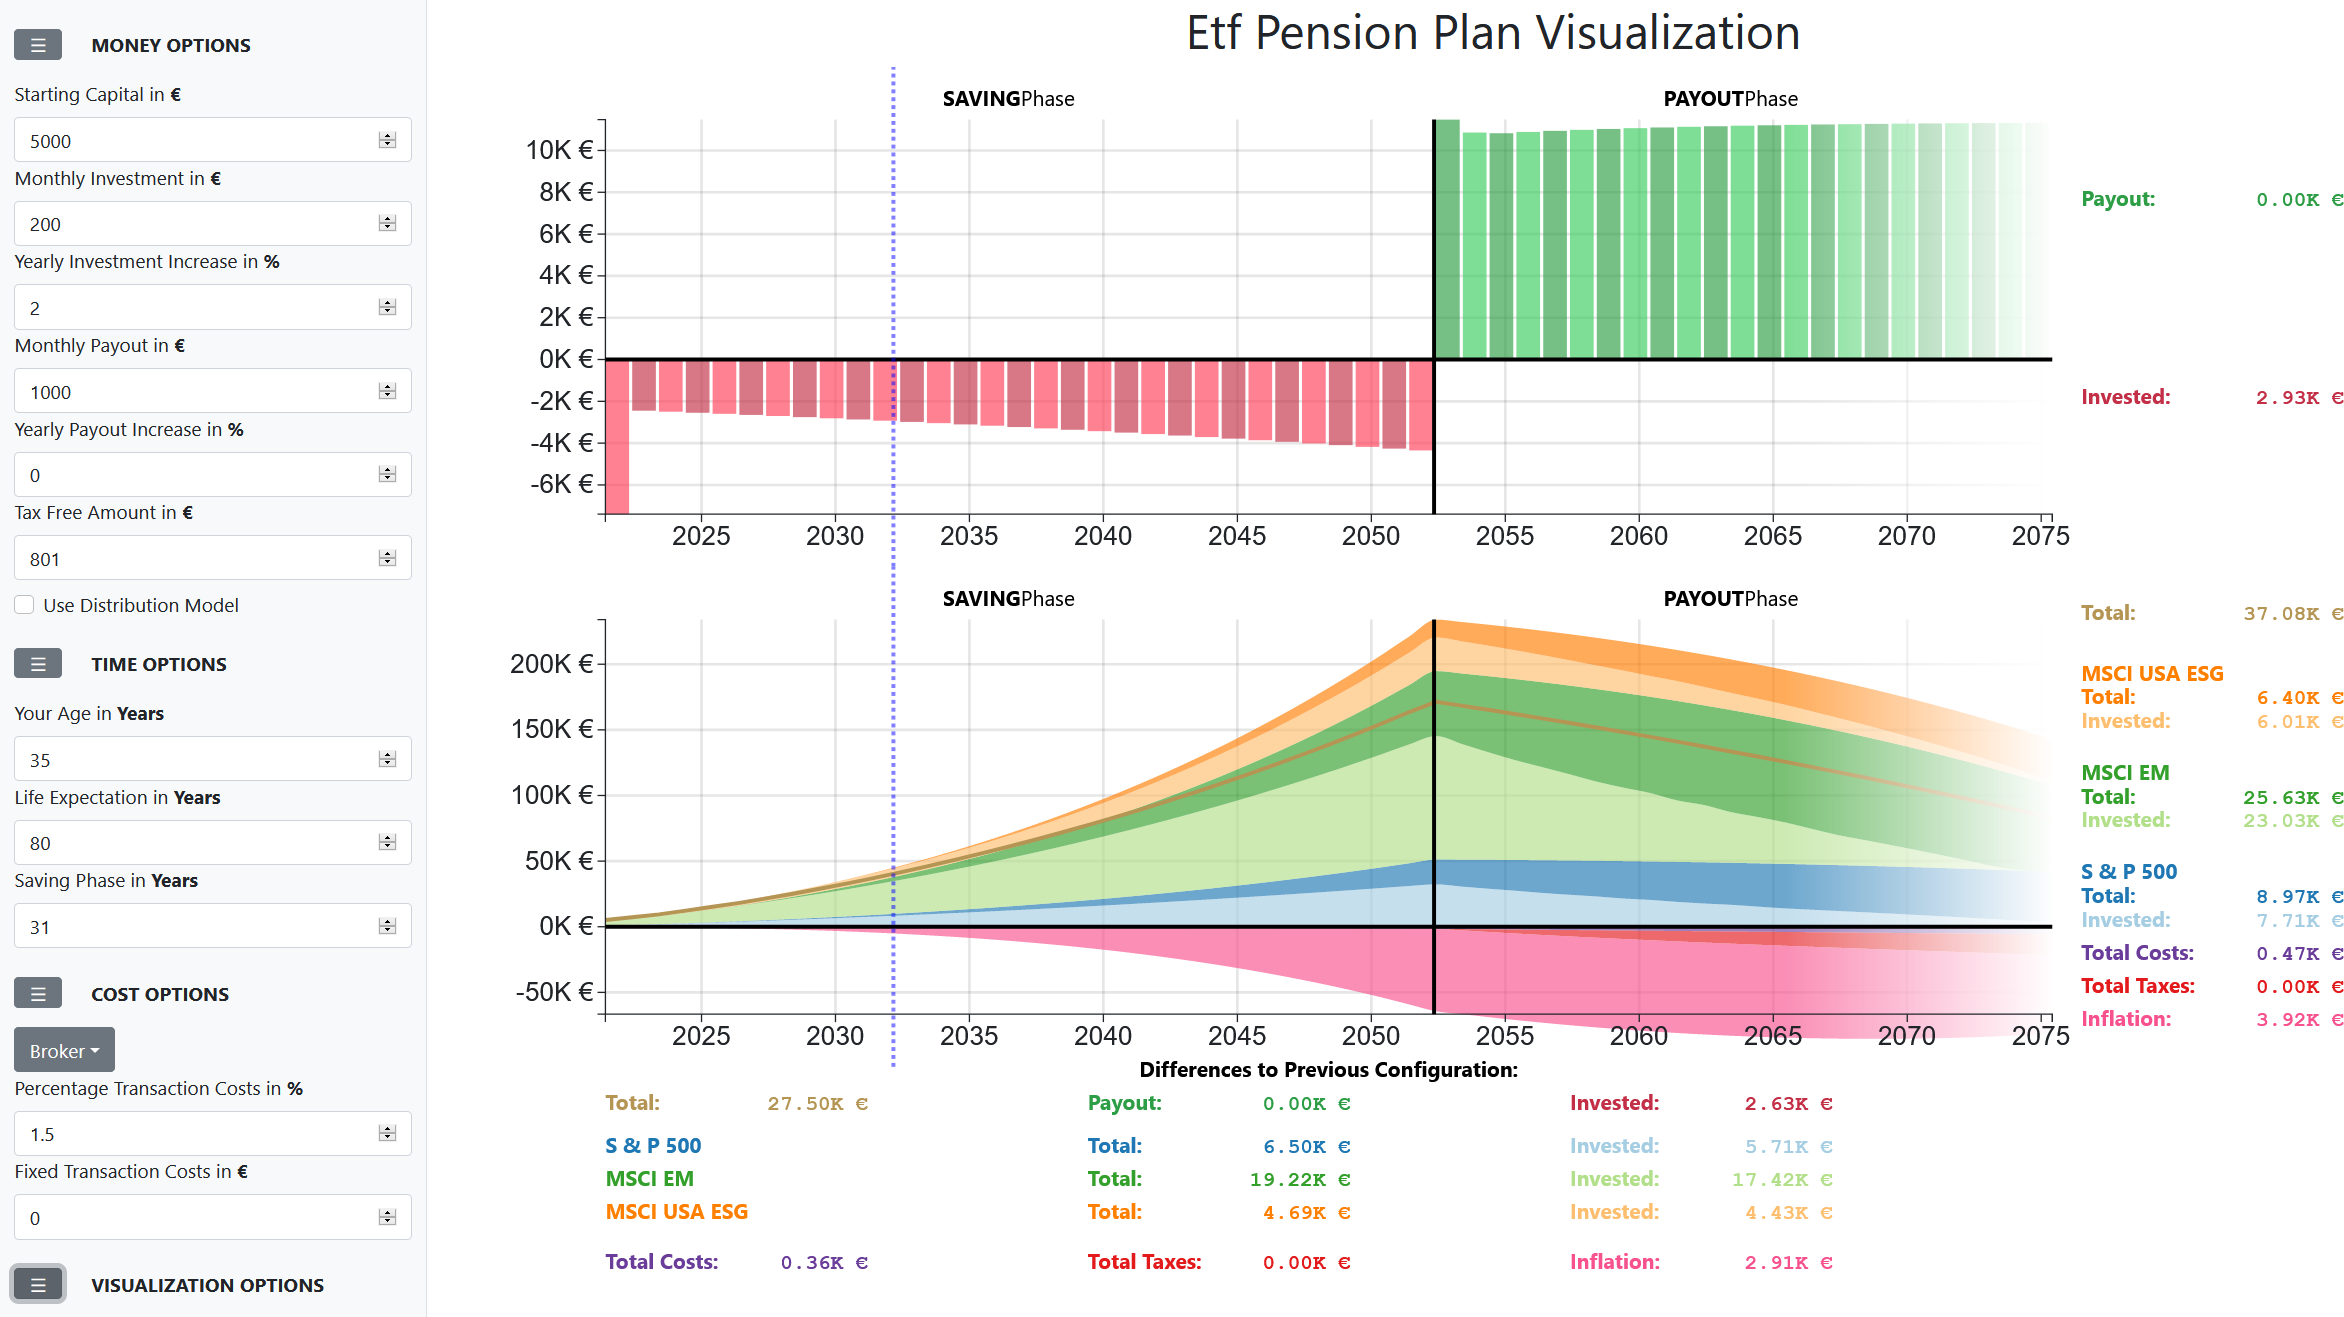
\includegraphics[width=\linewidth]{figures/visualization-full.png}
    \caption{A complete overview of the existing prototype. 
        A parameter pane divided into money, time, cost, and visualization options is on the left. 
        The cash flow chart (top) displays the yearly investments and payouts. 
        The depot chart (center) displays the forecast including costs, taxes, and inflation. 
        Details w.r.t. the year pointed at are displayed right next to each chart. 
        An agglomeration of all values is displayed in a tabular fashion (bottom).}
    \label{fig:visualization-full}
\end{figure}

\paragraph{Discussion}
The simulation has several advantages and a few disadvantages. 
First, it relies on a few recent years for forecasting.
This is hard to come by since ETFs have become popular only in recent years. 
Next, the simulation is deliberately using a linear model instead of an exponential model to prevent overestimation.
Moreover, the simulation is based on the current situation. 
Thus, it is based on the current taxation laws and broker costs. 
Both will probably change in the future, which would invalidate the simulation.
The visualization is good at displaying the negative factors costs, taxes and inflation, and the ratio between those negative factors and the depot value.
It covers both the depot development and the cash flow simultaneously. 
A drawback might be the unconventional layout of the inflation, which has been mentioned by several individuals who got in touch with the visualization.
The other negative values are already discounted from the depot value, except the inflation.
We decided to add a little hint by providing a visualization option that discounts the inflation from the total line.
In its presented state, the simulation and visualization are missing further explanations for the parameters. 
For now, the user is expected to have basic knowledge on ETFs and what factors are involved in a long-term savings plan or retirement strategy.
However, a certain learning and exploration phase is expected.
The user is expected to discover and understand the parameters and their effect on the simulation and visualization by means of iterative exploration of the problem and solution space.
A similar approach has been taken by~\cite{portfolio-charts}. 
There, a lot of different visualizations are offered, each, however, stands for itself and does not allow for direct visual transfer between one another.
We think that the visualization is a meaningful resource for individuals who intend to start ETF saving plans and want to understand the impact of certain strategies and figure out the specifics for their plan.
Furthermore, the visualization could be applied to other use cases, e.g., the passive income for one's children, which would be handed over to them when they are grown up.

\section{Conclusions}
We implemented a prototypical simulation and visualization for an ETF retirement plan strategy, which is based on the German cost and taxation model. 
The prototype (\href{https://etf-vis.net}{etf-vis.net}) is built using TypeScript, React, Bootstrap, and D3, and its source code (\href{https://github.com/varg-dev/etf-vis}{github.com/varg-dev/etf-vis}) is publicly available.
It can be used for different use cases next to the retirement planning such as planning a passive income for one's child.
It might be able to fill the gap of personal visualizations which can \enquote{support people with limited visualization literacy and analytics experience}~\cite{huang2015-personal} and, consequently, support understanding and actions to enact on one's own retirement plans~\cite{pandey2014-power}. 
As a result, we extend available literature towards what is needed to create effective, interactive visualization for the communication and literacy of upcoming financial products~\cite{lusardi2017-narratives}. 

In order to evaluate the effectiveness of the visualization, a user study with different groups regarding age, economic status and financial literacy could be done. 
The visualization could be extended to explain the underlying simulation. 
Moreover, the simulation could be extended with further components, such as a simulation of a financial crash. 
That way, a user could interactively explore the consequences on the retirement savings.
We believe that the type of visualization presented is a useful addition to the tools already available and facilitates the planning and adjustment of long-term savings goals and strategies.

\begin{acks}
    This work is part of the \enquote{Software-DNA} project, which is funded by the European Regional Development Fund (ERDF or EFRE in German) and the State of Brandenburg (ILB).
\end{acks}

\balance
\bibliographystyle{ACM-Reference-Format}
\bibliography{references}

\end{document}
\endinput
